\documentclass[10pt,hyperref={colorlinks,linkcolor=black,citecolor=blue!80,urlcolor=blue!60},handout]{beamer} %"handout" serveix per a treure els \pause
\usepackage[mode=buildnew]{standalone}
\usepackage[utf8]{inputenc}
\usepackage[catalan,english]{babel}
\usepackage{amsmath,amssymb}
\usepackage{tikz}
\usepackage{pgfplots}
\usepackage{graphicx}
\usepackage{subfig}
\usepackage{biblatex}
\usepackage{stmaryrd}
\usepackage{csquotes}

\usetheme{Copenhagen}
\usecolortheme{seahorse}

\addbibresource{references.bib}

\pgfplotsset{compat=newest}

%%%%%%%% colors %%%%%%%%
\definecolor{lessgreen}{RGB}{0,100,0}
\definecolor{color1}{RGB}{255,158,1}
\definecolor{color2}{RGB}{255,74,1}
\definecolor{color3}{RGB}{220,0,0}
%%%%%%%%%%%%%%%%%%%%%%%%

%%%%%%%%% setbeamer %%%%%%%%%
\setbeamersize{text margin left=0.5cm,text margin right=0.5cm}
\setbeamerfont{footnote}{size=\tiny}
\setbeamertemplate{bibliography item}[text]
%%%%%%%%%%%%%%%%%%%%%%%%%%%%%

%%%%%%%% newtheorems %%%%%%%%
\theoremstyle{definition}
\newtheorem{defin}[theorem]{Definició}
%%%%%%%%%%%%%%%%%%%%%%%%%%%%%

%%%%%%%% newcommands %%%%%%%%
\newcommand\enllas{\raise.5pt\hbox{$\boxempty\kern-4.85pt{}^{\nearrow}$}\kern-2pt}
\DeclareFieldFormat{url}{%
  \ifhyperref
    {\href{#1}{\enllas}}
    {\url{#1}}}% url symbol for references. It is needed \usepackage{stmaryrd}
\newcommand\Hz{\text{ Hz}}
\DeclareMathOperator{\diss}{diss}
\DeclareMathOperator{\arccosh}{arccosh}
%%%%%%%%%%%%%%%%%%%%%%%%%%%%%

\institute[UAB]{Taller de modelització\\
\vspace{5pt}Grau en Matemàtiques\\
\vspace{5pt}Universitat Autònoma de Barcelona}
\title[Mesures de dissonància]{Mesures de dissonància}
\author[Víctor, Oriol, Carlo]{Víctor Ballester\and Oriol Bosquet\and Carlo Sala}
\date{Maig 2021}

\begin{document}
\selectlanguage{catalan}
\frame{\titlepage}
\begin{frame}{Definicions prèvies}
    \begin{defin}[So simple]
        Un \textit{so simple} és una parella $(f,a)$ on $f$ és la freqüència del so i $a$ és l'amplitud d'aquest.
    \end{defin}
    \begin{defin}[So complex]
        Un \textit{so complex} (o nota musical) amb $n$ harmònics és una parella $(F,A)\in(\mathbb{R}^n)^2$ on $F = (f_1,\ldots,f_n)$ són les freqüències de cada un dels harmònics i $A = (a_1,\ldots,a_n)$ són les amplituds de cada un d'aquests.
    \end{defin} \pause
    \begin{defin}[Dissonància]
        Qualitat de dos o més sons amb una relació de freqüències concreta, que sonen poc agradables a l'oïda humana.
    \end{defin}
    \begin{defin}[Consonància]
        Qualitat de dos o més sons amb una relació de freqüències concreta, que sonen agradables a l'oïda humana.
    \end{defin}
\end{frame}
\begin{frame}{Primer model per a sons simples}
    Dissonància entre dues freqüències $f_1$ i $f_2$:
    $$\diss(r)=
        \left\{\begin{array}{lll}
            e^{\beta f_1(r-1+\gamma_{f_1})} & \text{si} & 0<r<1-\gamma_{f_1}\\
            \cosh\left[\frac{\arccosh(2)}{(\gamma_{f_1})^2}(r-1)^2\right]-1 & \text{si} & 1-\gamma_{f_1}<r<1+\gamma_{f_1}\vspace{5pt}\\
            e^{-\beta f_1(r-1-\gamma_{f_1})} & \text{si} & 1+\gamma_{f_1}<r
        \end{array}\right.$$ on $\beta$ és una constant i $\gamma_{f_1}\propto\frac{1}{f_1}$.\par\vspace{1cm}\pause
    \textbf{Inconsistències i problemes del model:}
    \begin{itemize}
        \item No dependència de $f_2/f_1$ $\implies$ Mal comportament a freqüències altes\pause
        \item Complexitat de la fórmula\pause
        \item No dependència de l'amplitud dels sons
    \end{itemize}
\end{frame}
\begin{frame}{Teoria auditiva}
Per tal d'introduir el nou model necessitem fer menció de \textbf{l'amplada de banda crítica}.\pause
\setcounter{subfigure}{0}
\begin{figure}
    \centering
    %\captionsetup[subfigure]{labelformat=empty}
    \subfloat[Còclea \href{https://www.pinterest.com/pin/336995984614355654/}{\enllas}]{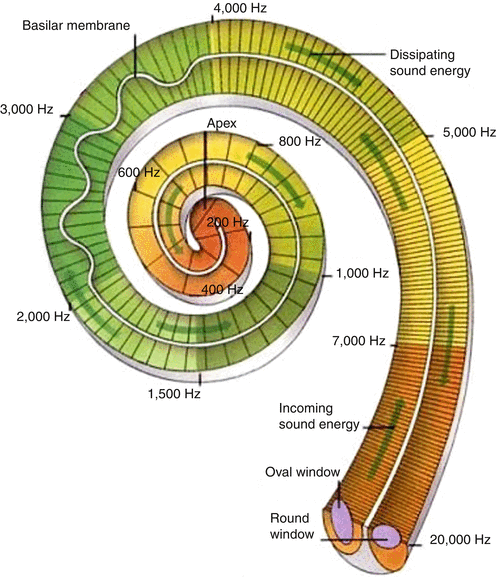
\includegraphics[height=3.2cm]{Imatges_beamer2/coclea.png}}\hspace{1cm}\pause
    \subfloat[Membrana basilar \href{https://www.phys.uconn.edu/~gibson/Notes/Section7_3/Sec7_3.htm}{\enllas}]{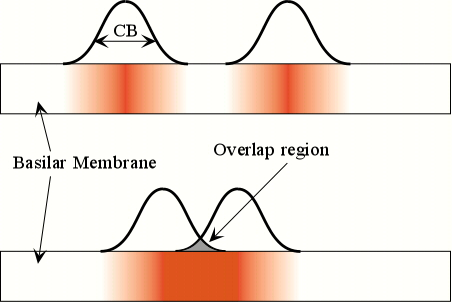
\includegraphics[height=3.2cm]{Imatges_beamer2/basilar_membrane.jpg}}
\end{figure}\pause 
\begin{itemize}
    \item Dues freqüències que vibren a la mateixa zona de la membrana basilar són \textbf{dissonants}. \pause
    \item Dues freqüències que no vibren a la mateixa zona de la membrana basilar són \textbf{consonants}. \pause
\end{itemize}
Parametrització de l'amplada de banda crítica \cite{hutchinson}:
\begin{equation*}
    \text{CBW}(f)=1.72 f^{0.65}
\end{equation*}
\end{frame}
\begin{frame}{Segon model per a sons simples}
    Plompt i Levelt \cite{plomp} van modelitzar empíricament les corbes de dissonància en relació amb la banda crítica.
    \begin{figure}
        \centering
        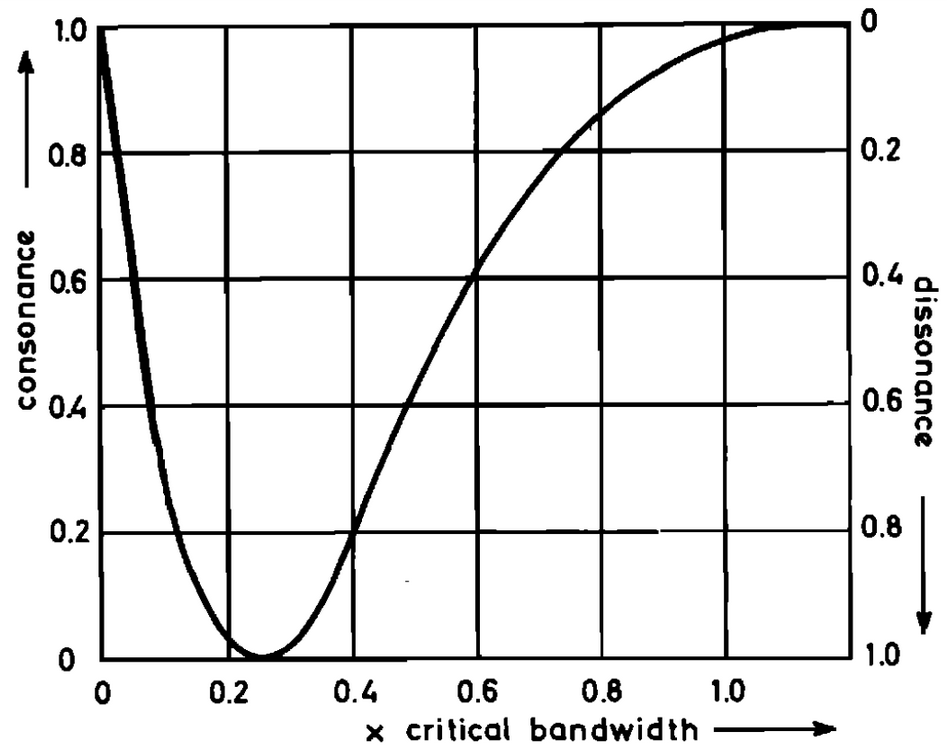
\includegraphics[width=5cm,angle=-0.1]{Imatges_beamer2/plompt-levelt.png}
        \caption{Resultats empírics de Plompt i Levelt \cite{plomp}}
    \end{figure}
    \only<1| handout:0>{\invisible{Algunes equacions que aproximen aquest tipus de funcions són: $$\delta_1(x)=e^{-\alpha x}-e^{-\beta x}\text{ \cite{sethares1}}\qquad\delta_2(x)=e^{-\left(\log(\beta x)\right)^2}\qquad\delta_3(x)=\beta xe^{-\beta x}$$}}
    \only<2| handout:1>{Algunes equacions que aproximen aquest tipus de funcions són: $$\delta_1(x)=e^{-\alpha x}-e^{-\beta x}\text{ \cite{sethares1}}\qquad\delta_2(x)=e^{-\left(\log(\beta x)\right)^2}\qquad\delta_3(x)=\beta xe^{-\beta x}$$}
    \hypersetup{citecolor=black!30}
    \only<3| handout:0>{Algunes equacions que aproximen aquest tipus de funcions són: $$\textcolor{black!20}{\delta_1(x)=e^{-\alpha x}-e^{-\beta x}\text{ \cite{sethares1}}\qquad\delta_2(x)=e^{-\left(\log(\beta x)\right)^2}}\qquad\delta_3(x)=\beta xe^{-\beta x}$$}\hypersetup{citecolor=blue!80}
\end{frame}
\begin{frame}
    Considerem dos sons simples $(f_1,a_1)$ i $(f_2,a_2)$:\pause
    $$\delta(x)\implies\delta(f_1,f_2,a_1,a_2)$$\par\pause
    Imposant:
    \begin{enumerate}
        \item $\max\delta(f_1,f_2,1,1)=1$ i que s'assoleixi quan $\frac{|f_1-f_2|}{\text{CBW}(f_m)}=0.25$, on $f_m=\frac{f_1+f_2}{2}$.\pause
        \item $\delta(f_1,f_2,a_1,a_2)\propto a_1a_2$\pause
    \end{enumerate}
    Resulta:
    \begin{equation*}
        \delta(f_1,f_2,a_1,a_2)=a_1a_2\frac{|f_2-f_1|}{\text{CBW}(f_m)\cdot 0.25}e^{1-\frac{|f_2-f_1|}{\text{CBW}(f_m)\cdot 0.25}}
    \end{equation*}
    \begin{figure}
        \centering
        \includestandalone[mode=image|tex,width=5.5cm]{Imatges_main/model2}
    \end{figure}
\end{frame}
\begin{frame}{Model per a sons complexos}
    Considerem dos sons complexos $\mathcal{S}_1=(F_1, A_1)\in(\mathbb{R}^{n_1})^2$ i $\mathcal{S}_2=(F_2, A_2)\in(\mathbb{R}^{n_2})^2$:
    \begin{gather*}
        F_1=(f_1,2f_1,\ldots, n_1f_1)\qquad A_1=(a_1,\ldots, a_{n_1})\\ F_2=(f_2,2f_2,\ldots, n_2f_2)\qquad A_2=(a_1,\ldots, a_{n_2})
    \end{gather*}\pause
    Si definim $D(\mathcal{S}_k)$ (dissonància intrínseca) com: $$D(\mathcal{S}_k)=D((F_k, A_k))=\sum_{i=1}^{n_k}\sum_{j=i}^{n_k}\delta(if_k, jf_k, a_k, a_k)$$\pause
    I $D(\mathcal{S}_1, \mathcal{S}_2)$ (dissonància comú) com: $$D(\mathcal{S}_1, \mathcal{S}_2)=D((F_1, A_1), (F_2, A_2))=\sum_{i=1}^{n_1}\sum_{j=1}^{n_2}\delta(if_1, jf_2, a_i, a_j)$$\pause
    \textbf{Dissonància total $\mathcal{D}(\mathcal{S}_1, \mathcal{S}_2)$:}
    \begin{equation*}
        \mathcal{D}(\mathcal{S}_1, \mathcal{S}_2)=D(\mathcal{S}_1)+D(\mathcal{S}_2)+D(\mathcal{S}_1, \mathcal{S}_2).
    \end{equation*}
\end{frame}
\begin{frame}
    Si considerem $n_1=n_2=7$, $a_k=\frac{1}{k^{0.4}}$ i fixem $f_1=440\Hz$:\pause
    \begin{figure}
        \centering
        \includestandalone[mode=image|tex,width=9cm]{Imatges_main/complex2}
    \end{figure}
\end{frame}
\begin{frame}{Aclariment}
    Diferència entre sons simples i sons complexos:
    \begin{table}[ht]
        \centering
        \begin{tabular}{cc@{\hspace{0.5\tabcolsep}} cc@{\hspace{0.5\tabcolsep}} cc@{\hspace{0.5\tabcolsep}} c}
        & \multicolumn{2}{c}{$f_2=466.16\Hz$} & \multicolumn{2}{c}{$f_2=659.26\Hz$} & \multicolumn{2}{c}{$f_2=847\Hz$}\\
        So simple  & \beamerbutton{Play} & dissonant & \beamerbutton{Play} & ``no dissonant" & \beamerbutton{Play} & ``no dissonant"\\
        So complex & & & \beamerbutton{Play} & consonant & \beamerbutton{Play} & dissonant 
        \end{tabular}
    \end{table}
    \setcounter{subfigure}{0}
    \begin{figure}[ht]
        \centering
        \subfloat[Sons simples]{\includestandalone[mode=image|tex,width=5.9cm]{Imatges_beamer2/simple440}}
        \subfloat[Sons complexos]{\includestandalone[mode=image|tex,width=5.9cm]{Imatges_beamer2/complex440}}
    \end{figure}
\end{frame}
\begin{frame}{Verificació del model}
    Per tal de verificar el nostre model hem dut a terme un test. \pause
    \begin{itemize}
        \item Cada persona valorava el seu nivell musical (molt baix, baix, intermedi, alt o molt alt).\pause
        \item Hi havia 11 combinacions de dos sons complexos.\pause
        \item S'havia de qualificar cada so d'1 (molt dissonant) a 10 (molt consonant).
    \end{itemize}\pause
    En total vam aconseguir 190 respostes.
    \begin{figure}
        \centering
        \includegraphics[width=5.45cm]{Imatges_main/mediana.tex}
    \end{figure}
\end{frame}
\begin{frame}{Refinaments}
    Possibles millores:\pause
    \begin{itemize}
        \item Generalització de la fórmula per un nombre arbitrari de sons: $$\mathcal{D}(\mathcal{S}_1,\mathcal{S}_2)\implies\mathcal{D}(\mathcal{S}_1,\mathcal{S}_2,\ldots,\mathcal{S}_n)\text{\pause}$$
        \item Considerar sons no harmònics\pause
        \item Millorar la fiabilitat del test
    \end{itemize}
\end{frame}
\begin{frame}[noframenumbering]{Referències}
    \printbibliography[heading=none]
\end{frame}
\end{document}